\section {Simulation Description}

A program will be developed that will simulate air traffic in the United States. In order to do this,
rules for flight must be developed. This includes airport runway operation rules, and rules for
inter-region travel.

Maximum Throughput Capacity (MTC) is the fundamental measure of the capacity of the
runway. It is measured in movements (arrivals and departures) per hour. The most significant
factor affecting capacity is spacing between successive aircraft in both takeoff and landing
streams. Of course, there are many factors that play a role in determining capacity. Runway
system capacity depends on:


\begin{itemize}
\renewcommand{\labelitemi}{$\bullet$}
\item Runway configuration
\item Environment on which aircraft operate (wind level, cloud ceiling)
\item Availability of NAVAIDS \& ATC facilities and operating requirements/standards
\item Characteristics of demand
\item Other air traffic control rules
\end{itemize}

There are many flight rules that can be considered in the development of a simulation. Among
these include minimum following distances for different aircraft sizes, minimum following
distances depending on weather conditions and navigation equipment, amount of time required
to take-off and land, and minimum amounts of time between successive take-offs and landings \cite{fed1}.
However, for the simplicity of this simulation, it will be assumed that all aircraft are the same
size, have the same up-to-date navigation equipment and will all operate alike. Because of the
complexity of implementing many of these flight rules, a single minimum assumed time-space
gap will be considered for all departing and arriving aircraft. Also, it is assumed that there will be
sufficient airspace such that collisions between aircraft will be avoided while en route.

The location of airports within a region and individual airport characteristics must be determined.
Only airports designated as primary commercial airports will be considered for this simulation.
This includes airports with more than 10000 yearly enplanements. Furthermore, there are four
airport sizes, as designated by the percentage of all US enplanements as shown in table \ref{table:airport_size} \cite{fed2}.

\begin{table}[h]
\begin{center}
\addtolength{\tabcolsep}{-0pt}
%\tiny
\caption{Hub type Enplanement Definitions}
\label{table:airport_size}
\begin{tabular}{|c|c|}\hline

Hub Type & Enplanements  \\\hline
Large & Greater than 1\%  \\\hline
Medium & 0.25 - 1\%  \\\hline
small & 0.05 - 0.25 \% \\\hline
Non-Hub & Less than 0.05 \%  \\\hline

\end{tabular}
\end{center}
\end{table}

Many airports have runways that cross each other for variable wind conditions - these runways
are never used at the same time. For the simplicity of our simulation, and due to the difficulty of
finding airport runway orientations, it is assumed that the wind direction does not play a role in
the number of useable runways, and that planes will be able to takeoff/land in the direction of
the orientation of the maximum number of useable runways). A survey of different airport types
reveals the distribution of the maximum number of runways that can be used concurrently in the following table:

\begin{table}[htb]
\begin{center}
\addtolength{\tabcolsep}{-0pt}
%\tiny
\caption{Airport Number of Runways}
\label{table:airport_runway}
\begin{tabular}{|c|c|}\hline

Hub Type & Runways  \\\hline
Large & 2 - 6  \\\hline
Medium & 1 - 3  \\\hline
small & 1 - 2 \\\hline
Non-Hub & 1  \\\hline

\end{tabular}
\end{center}
\end{table}


Knowing the number of enplanements at each airport will be particularly useful in determining
the number of flights expected to take-off and land from a particular airport. Also, knowing the
number of runways each airport has will be important in determining capacity of that airport.
There is expected to be a correlation between the number of runways and the number of
enplanements (demand and capacity).

Air traffic control is divided into 20 regions in the continental United States. Given a list of 328
primary commercial service airports from the Federal Aviation Administration, each airport was
placed into its appropriate region.

\begin{figure} [htb]
\centering
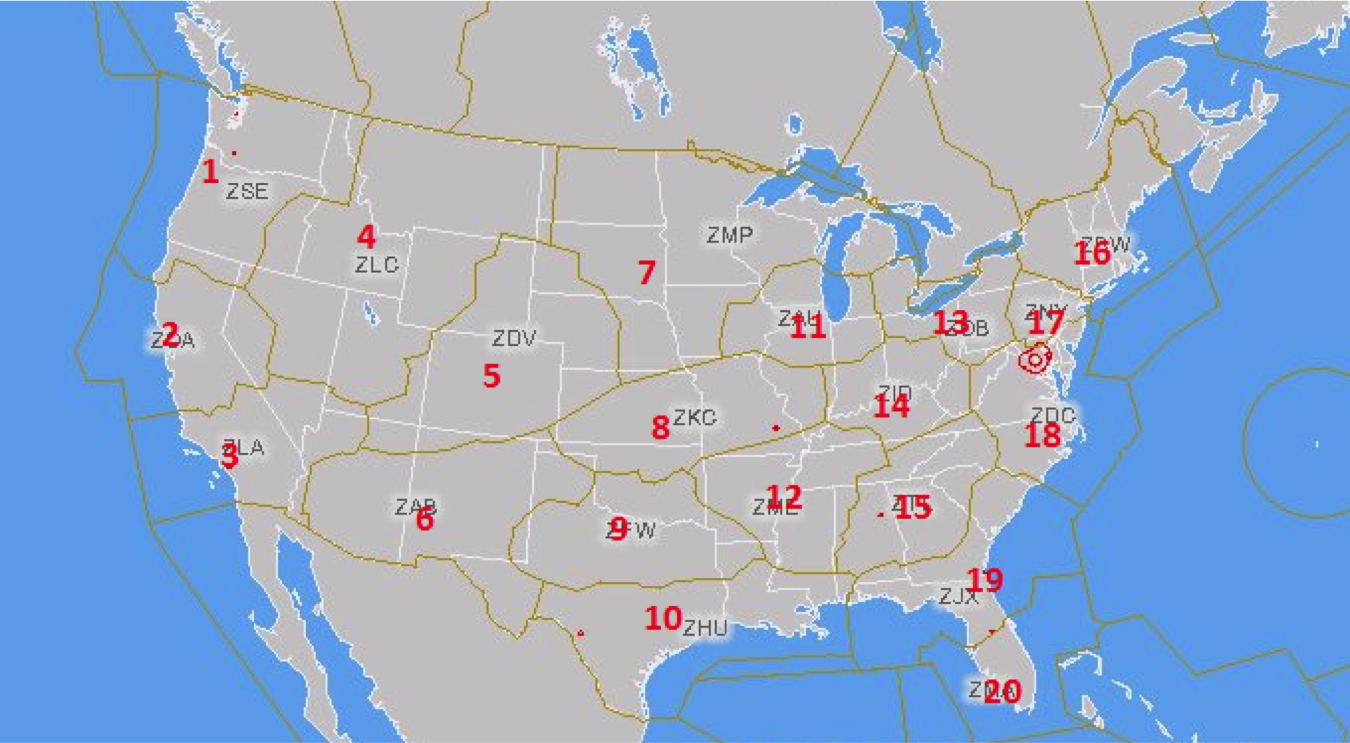
\includegraphics[width=3in]{/Users/chayong/Dropbox/dsrt_2012/figs/map.png}
\caption{Location of Airport Region}
\label{fig:airport_region}
\end{figure}


Once the number or airports in each region was determined, a region size (based on the
distribution of airport types within that region) could be assigned. More weight was given to
regions that had more large hubs, and less emphasis was placed on non-hub airports.
Figure \ref{fig:airport_region} shows the distribution of airport types for all 20 regions.

\begin{table} [htb]
\begin{center}
\addtolength{\tabcolsep}{-0pt}
\tiny
\caption{Regional Airport Distribution}
\label{table:regional_airport_dist}
\begin{tabular}{|c|c|c|c|c|c|c|c|c|c|c|c|c|c|}\hline

Region & L & M & S & N & Total & Region Size & Region & L & M & S & N & Total & Region Size  \\\hline
1 & 1 & 1 & 1 & 16 & 19 & M & 11 & 2 & 1 & 3 & 7 & 13 & M  \\\hline
2 & 1 & 4 & 1 & 9 & 15 & M & 12 & 0 & 2 & 3 & 7 & 12 & S  \\\hline
3 & 3 & 3 & 3 & 10 & 19 & L & 13 & 1 & 3 & 4 & 9 & 17 & M  \\\hline
4 & 1 & 0 & 2 & 17 & 20 & M & 14 & 1 & 2 & 4 & 4 & 11 & S  \\\hline
5 & 1 & 0 & 1 & 15 & 17 & S & 15 & 2 & 0 & 5 & 8 & 15 & M  \\\hline
6 & 0 & 1 & 2 & 2  & 5 & S & 16 & 3 & 3 & 6 & 13 & 25 & L  \\\hline
7 & 1 & 1 & 4 & 28 & 34 & L & 17 & 2 & 0 & 2 & 4 & 8 & S  \\\hline
8 & 1 & 3 & 3 & 11 & 18 & L & 18 & 3 & 2 & 3 & 8 & 16 & L  \\\hline
9 & 1 & 1 & 3 & 9 & 14 & S & 19 & 1 & 1 & 7 & 10 & 19 & M  \\\hline
10 & 1 & 4 & 3 & 13 & 21 & L & 20 & 3 & 2 & 1 & 4 & 10 & M  \\\hline
\end{tabular}
\end{center}
\end{table}

For the simulation, the size of a region is equivalent to the number of aircraft that can be in
that region’s airspace at a given time. If airspace capacity has been reached, no aircraft may
enter that region’s airspace from another region, or take off from an airport in that region until
another plane has exited the region or landed at an airport in that region. If an aircraft attempts
to enter a region (a request), but cannot due to capacity constraints, this is considered a
request rejection. The aircraft will have to make another request at the conclusion of the next
event. Thus, queues form at airports (for planes waiting to take off) and at boundaries between
regions. The effectiveness of air traffic operations can be estimated by analyzing the total
number of events and the number of rejected requests (due to the fact that a runway is in use or
an air traffic control region is at capacity).

Lastly, it will be important to describe inter-regional travel. To do this, spatial relationships must
be made between neighboring regions. Approximate distance between central locations in
neighboring regions are shown in figure \ref{fig:approx_dist}.

\begin{figure} [htb]
\centering
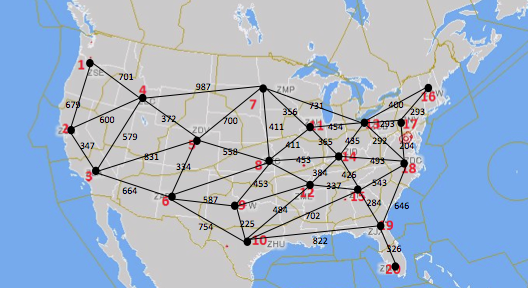
\includegraphics[width=3in]{figs/map_graph.png}
\caption{Approximate Distance Between Central Locations}
\label{fig:approx_dist}
\end{figure}

The total distance an aircraft travels from one region to another can be determined by finding
a path from the figure above. Because it is of interest for aircraft to take the shortest possible
route, Dijkstra’s algorithm is applied to determine a plane’s route from one region to another.


